\documentclass[letterpaper,12pt]{article}

\usepackage{tabularx} % extra features for tabular environment
\usepackage{amsmath}  % improve math presentation
\usepackage{graphicx} % takes care of graphic including machinery
\usepackage[margin=1in,letterpaper]{geometry} % decreases margins
\usepackage[final]{hyperref} % adds hyper links inside the generated pdf file
\hypersetup{
	colorlinks=true,       % false: boxed links; true: colored links
	linkcolor=blue,        % color of internal links
	citecolor=blue,        % color of links to bibliography
	filecolor=magenta,     % color of file links
	urlcolor=blue         
}
\usepackage{blindtext}
\usepackage{pdfpages}

\usepackage{xcolor}
\usepackage{listings}

\colorlet{mygray}{black!30}
\colorlet{mygreen}{green!60!blue}
\colorlet{mymauve}{red!60!blue}

\lstset{
	backgroundcolor=\color{gray!10},  
	basicstyle=\ttfamily,
	columns=fullflexible,
	breakatwhitespace=false,      
	breaklines=true,                
	captionpos=b,                    
	commentstyle=\color{mygreen}, 
	extendedchars=true,              
	frame=single,                   
	keepspaces=true,             
	keywordstyle=\color{blue},      
	language=c++,                 
	numbers=none,                
	numbersep=5pt,                   
	numberstyle=\tiny\color{blue}, 
	rulecolor=\color{mygray},        
	showspaces=false,               
	showtabs=false,                 
	stepnumber=5,                  
	stringstyle=\color{mymauve},    
	tabsize=3,                      
	title=\lstname                
}

%++++++++++++++++++++++++++++++++++++++++


\begin{document}
	
	\title{ECE1754 Project Report}
	\author{Behrooz Zarebavani}
	\date{\today}
	\maketitle
	\section{Abstract}
	
	
	Compiler transformations, especially loop transformations, play a significant role in improving the runtime of many time-intensive kernels. As a result, guaranteeing the correctness of these transformations play an important role. There are three major approaches to prove the correctness of the program. I) proof of equivalence of affine programs, II) Matching the execution trace, and III) checking the output of the program via testing. All of these approaches have their flaws, and Polycheck attempt to solve these problems by combining a runtime check with the power of trace checking. In what follows, I will implement a demo of their first algorithm (Algorithm A in the paper) and evaluate a transformation to see whether it can detect errors that the testbench that I am using cannot detect.
	
	
	\section{Introduction}
	
	When a code is transformed, typically, it is not like the original code at all. Experts use automatic testing via a choice of a dataset to prove that their transformation is correct. However, in many cases, this may backfire. Imagine a matrix-matrix multiplication with zero matrices as an input. Thus, any code that generates zero az output can be assumed to be correct.

	For addressing this data-dependence problem, automatic equivalence checking techniques such as static verification are introduced. This technique proved to be hard to use and requires a solid mathematical foundation and programming techniques. Also, it is constrained by the type of program that it can verify. For example, if the program is non-affine, it will have a hard time proving the code's correctness.
	
	To address this problem, that both codes should be affine, experts come up with trace-based matching. That is, the trace of the two programs should be matched entirely. An example of this technique is in~\cite{schordan2014verification}. The disadvantage of this method is the space of the trace. Usually, this space is enormous and requires a significant amount of time to be checked and generated (please consider a huge graph matching problem). Polycheck~~\cite{bao2016polycheck} tries to address these problems by combining the trace idea with the runtime check. It instruments the code with some assertions which identify any deviation in the data-dependency flow. After retrieving their code, I realized that they use the PoCC compiler, which is the result of many previous scientific works like~\cite{LOECHNER1999POLYLIB} and an integer set programming library, namely ISL~\cite{VERDOOLAEGE2010ISL}, combined with ROSE~\cite{quinlan2000rose} compiler. Since it was hard for me to learn all of them (and I was in the middle of my implementation), I decided to choose the ROSE entirely. Thus, since it was my first attempted to get familiar with a compiler, I believe that I missed multiple corner cases, so this work is limited. But it was a great experiment for me to learn and think of the code the way a compiler is seeing it. After some simplification, in this work, I am presenting a ROSE pass that reads the code. Using some predefined libraries, it will instrument the code and verify the correctness of a transformation. The milestones are as follow:
	
	\begin{itemize}
		\item Implementation of four general function (firstWriter, nextWriter, writeBeforeRead, and lastWriter) and infrastructure to work with these functions resulted in polycheck\_demo\_functions.h header file.
		\item Computation of the original schedule of the code~\cite{feautrier1992some}
		\item Computation of the required mapping between dataspace and iteration space using ROSE compiler
		\item Instrumentation of the code with right helper variables, initialization of these variables and their usage using ROSE compiler
	\end{itemize}
	
	
	
	\section{Methods}
	
 A transformed program is declared to be equivalent to an input	program if I) the statement instances in the transformed program can be mapped in a bijective, or one-to-one, fashion to statement instances in the input program, and II) each statement instance in such a bijection satisfies the same dependencies as in the input program. 

Since I simplify the problem to use only one statement, we can assume that we only have to check the dependencies constraints. To do that, we assign a shadow variable to each data space of the program. These shadow variables will store the last statement instance that \b{write} to their corresponding data space. Then, we can use this information and the original schedule of the input program to check the dependency constraints.

To clarify, please consider the original code in listing~\ref{code:original}. After transforming the code using a recursive function that imitates the tiling approach, we will have the transformed code in listing~\ref{code:transformed}. Now, we first have to do a light analysis on the original code. This analysis involves computing the original schedule used as the statement instance form $S<t,i,j>$. Please note that the schedule computation describes in the implementation methods works for arbitrary code and an arbitrary number of statements. However, for the use in this demo, I will abstract that general view that is $S<0,t,0,i,0,j,0>$ into the $S<t,i,j>$. 

After original schedule computation, we will drive some mapping between iteration space and data space. For example a mapping like $\left( \begin{smallmatrix} 1&0\\ 0&1 \end{smallmatrix} \right) \times  \left( \begin{smallmatrix} i\\ j \end{smallmatrix} \right) + \left( \begin{smallmatrix} -1\\ 0 \end{smallmatrix} \right)$ drives the data reference subscripts of A[i - 1][j].
    \newpage

    \begin{lstlisting}[caption={The original code}, label={code:original}, captionpos=b]
void Original_Sidel()
	for(int t = 0; t < T; t++)
		for(int i = 1; i < N; i++)
			for(int j = 1; j < N; j++)
				A[i][j] = A[i - 1][j] + A[i][j - 1];
    \end{lstlisting}
    

    	 After driving these mapping and the original schedule, we will instrument the Transformed\_Sidel function with specific assertion to check whether the code complies to data dependency or not.
    \begin{lstlisting}[caption={The transformed code}, label={code:transformed}, captionpos=b]
void Transformed_Sidel(int t,int ilo,int ihi, int jlo, int jhi){
	if (ilo > ihi || jlo > jhi) return;
	if (ilo == ihi && jlo == jhi){
		A[ilo][jlo] = A[ilo-1][jlo] + A[ilo][jlo-1];
	}else{
		Transformed_Sidel(t, ilo,(ilo + ihi) / 2, jlo, (jlo + jhi)/2); //Top-Left
		Transformed_Sidel(t, ilo,(ilo + ihi) / 2, (jlo + jhi) / 2 + 1,jhi); //Top-Right
		Transformed_Sidel(t, (ilo + ihi) / 2 + 1, ihi, jlo, (jlo + jhi) / 2); //Bottom-Left
		Transformed_Sidel(t, (ilo + ihi) / 2 + 1, ihi, (jlo + jhi)/2 + 1, jhi); //Bottom-Right
	}
	if (ilo == 1 && ihi == N - 1 && jlo == 1 && jhi == N-1 && t < (T - 1)){
		Transformed_Sidel(t+1, ilo, ihi, jlo, jhi);// Next time step
	}
}
    \end{lstlisting}
    
    To describe this part, lets assume that an unknown statement instance in the transformed code will result in following statement A[a][b] = A[c][d] + A[f][h]. First, using the shadow(A[a][b]) and (a,b) we will map the current statement instance to a statement instance in the original code. For example assume that a = 5, b = 7 and the last statement instance that write to this address, namely A[5][7], stored in shadow(A[a][b]) is $S<1,5,7>$. Based on the original schedule and (a,b) we can determine that the current statement instance should be $S<2,5,7>$. 
  
  Now using the current statement instance, we will regenerate the whole statement instance that implies $S<2,5,7>$. That is using the mapping that we derived in compile time we will generate the following statement instance A[5][7] = A[4][7] + A[5][6]. At this point we should check whether the current statement A[a][b] = A[c][d] + A[f][h] is valid or not. That is assert(c == 4), assert=(d == 7), assert(f == 5) and assert(h == 6).
  
  After verifying that the statement is reading from the right places and write into the correct space, we need to check the values of the read data spaces. We should check whether the last statement instance that writes into these places is valid. To do that, we again get the current statement instance computed from the previous step, which is $S<2,5,7>$. Then passing the read data space and this statement instance to a function f($S<2,5,7>, (c,d)$), we can drive the last statement instance that was supposed to write in A[c][d], which is before $S<2,5,7>$. In here, it would be $S<2,4,7>$. Then we will check this with the shadow(A[c=4][d=7]). If they were the same, the data is valid. We also do the same thing for A[f][h]. 
  
  That is the basic idea. The rest of the implementation details will be describe in the Implementation section.
  
 
    
	
	\section{Implementation}
	\subsection{Main Function}
	I will start to explain the whole implementation, using the demo code, and function by function. So, for start, please see the main function in listing~\ref{code:main}.
	
	\subsubsection{Compiler code structure}
	
	 \begin{lstlisting}[caption={The core function that does the instrumentation in ROSE code}, label={code:compiler_main_function}, captionpos=b]
	void PolyCheckInstrumentation::startInstrumenting(){
	//Add Header
	addInstrumentationHeader();
	//Add Variables definitions
	definePolyCheckGlobalVariables();
	//initialize the Variables (extracting the statement information and initialize the shadow variable)
	initPolyCheckVariables();
	//Also add required assertions
	instrumentCode();
	}
	\end{lstlisting}
	
	
	Since the report has limited space, I will briefly explain the core compiler implementations. Please see~listing~\ref{code:compiler_main_function}. The instrumentation class in my code, has 4 main functions. the "addInstrumentationHeader" will add the polycheck\_demo\_functions.h which contain the 4 functions that I am using for data dependency checks. For that, I am using "SageInterface::insertHeader" and I add this header into the global scope.
	
	Then I need to define some global variables using "definePolyCheckGlobalVariables". To do that I am using "SageInterface::addTextForUnparser" interface and add the variables into the global scope.
	
	Now the most important function in this implementation is "initPolyCheckVariables" which initialize the require variables by analyzing the input code. The implementation details is a bit repetitive. So to simplify, I basically generate a simple AST graph with a toy example. Then I just see the required nodes characteristics like their parents, the operations that I allowed them to take, etc. To do that, I have used "NodeQuery::querySubTree" interface extensively and iterate over the nodes inside the tree. I also implemented some general codes to attach original schedule and print statements. However, later, I find out that functions "unparseToString" exist to just implement these for me. Also, at some point, I noticed that generalization is just getting worse when I proceed, so I end-up leaving some of my general implementations and stick to the simplified one. Because there where no use of them. 
	
	\begin{lstlisting}[caption={The main function of the hand instrumented code}, label={code:main}, captionpos=b, numbers=left,
	stepnumber=1]
int main() {
	//======================= Compiler stuff =======================
	std::vector<std::vector<bool>> readWriteSet(N, std::vector<bool>(N, true));//True for read set and False for the write set

	//Initialize Shadow variables
	for(int i = 1; i < N; i++){
		for(int j = 1; j < N; j++){
			//WriteSet
			if(readWriteSet[i][j]){//Write ref
				shadow[i][j].invalidate();
				shadow[i][j].makeNoInit();
				readWriteSet[i][j] = false;
			}
	
			if(readWriteSet[i - 1][j]){//Read ref
				shadow[i - 1][j].makeValid();
				shadow[i - 1][j].makeInit();
				readWriteSet[i - 1][j] = false;
			}
	
			if(readWriteSet[i][j - 1]){//Read ref
				shadow[i][j - 1].makeValid();
				shadow[i][j - 1].makeInit();
				readWriteSet[i][j - 1] = false;
			}
		}
	}

	//Initialize Mapping
	mapping.LHS_MAP.push_back(std::vector<int> {1, 0}); // Mapping for first subscript
	mapping.LHS_MAP.push_back(std::vector<int> {0, 1}); // Mapping for second subscript
	
	mapping.RHS_MAP.push_back(std::vector<int>({0, 1, 0}));
	mapping.RHS_MAP.push_back(std::vector<int>({0, 0, 1}));
	mapping.RHS_MAP.push_back(std::vector<int>({0, 1, 0}));
	mapping.RHS_MAP.push_back(std::vector<int>({0, 0, 1}));
	
	//Compute Bounds
	min_bound.instance.resize(3);
	min_bound.instance[0] = 0;
	min_bound.instance[1] = 1;
	min_bound.instance[2] = 1;
	min_bound.makeValid();
	
	max_bound.instance.resize(3);
	max_bound.instance[0] = T;
	max_bound.instance[1] = N;
	max_bound.instance[2] = N;
	max_bound.makeValid();
	
	//Compute wref related invariants
	wref_fix_flag.push_back(false);
	wref_fix_flag.push_back(true);
	wref_fix_flag.push_back(true);
	
	//Extract constants from the read reference
	read_const.push_back(-1);
	read_const.push_back(0);
	read_const.push_back(0);
	read_const.push_back(-1);
	//=========================== Test Section ======================
	//Generate some random data for Seidel
	std::random_device rd;
	std::mt19937 mt(rd());
	std::uniform_real_distribution<double> dist(1.0, 10.0);
	for(int i = 0; i < N; i++){
		for(int j = 0; j < N; j++){
			Original_A[i][j] = dist(mt);
			Transformed_A[i][j] = Original_A[i][j];
			Instrument_A[i][j] = Original_A[i][j];
		}
	}
	Original_Seidel();
	Transformed_Seidel(0, 1, N - 1, 1, N - 1);
	Instrumented_Seidel(0, 1, N - 1, 1, N - 1);
	for(int i = 0; i < N; i++){
		for(int j = 0; j < N; j++){
			if(Original_A[i][j] != Transformed_A[i][j])
				std::cout << "There is a problem in testing" << std::endl;
		}
	}
	
	//======================= Compiler stuff =======================
	//Last Writer Stuff Mapping
	for(int i = 1; i < N; i++){
		for(int j = 1; j < N; j++){
			std::vector<int> wref{i,j};
			assert(shadow[i][j] == polyfunc::lastWriter(max_bound,
			wref, wref_fix_flag, mapping.LHS_MAP));
		}
	}
	//================================================================
	
	
	return 0;
}
	\end{lstlisting}

	\subsubsection{Initializing shadow variables}
	
	
	Line 5-27 is about initializing shadow variables. The data space of a program, in the beginning, has two conditions. First, we either write to it at the beginning (like A[1][1] in listing~\ref{code:original} ) or we read from it at the beginning (like A[0][1] in listing~\ref{code:original}). To implement this part, we assume that the data space is rectangular. Thus, we make this initialization by dividing the statement into its write reference and read references (like the original statement). The tricky part is to find the induction variables that affect the statement to generate the for loops. Here from the three variables of the statement instance $S<t,i,j>$, we only need "i" and j loops. This isn't a very scientific approach, but I should have simplified some assumptions to make the implementation manageable. 

	First, we extract the write references and read references affine functions in "initPolyCheckVariables" to initialize the shadow variable. Then, we make sure that the statement is invalid for the write reference and cannot be read from any other statement instance. For the data space that we will read from them, I will make them valid and put the init statement inside them. The init statement is for further initialization steps. The valid flag is a flag that detects many other situations that may generate invalid statement instances. 

	
	\subsubsection{Mapping}
	
	Line 30-36 relates to the required mapping. To compute the mapping part, we need two things. First, a mapping from the data space to the related iteration space, e.g., in the listing~\ref{code:original} we need a mapping from write reference to the related iteration space (i,j). Then we also need a mapping from the iteration spaces to the reading space. To implement this part using ROSE, we assume that each subscript is in the form of a linear function of a * t + b * i + c * j + ... + d. Then we extract a, b, c ..., and d. Using these variables, we will drive the required mapping. For example for iterations space to first read reference A[i - 1][j], we simply need to dot product (0, 1, 0) with (t, i, j) + (-1) to drive the read reference of [i - 1].
	
	\subsubsection{min\_bound, max\_bound, wref\_fix\_flag, read\_const}
	Variables defined in lines 39 to 60 are going to be used to input the functions of Polycheck. Their initialization is trivial and can be computed efficiently using the previous steps' implementations.
	
	\subsubsection{Test function}
	Line 61-82 relates to initializing the array and running the two functions, and comparing their results. It initializes the array with some random variable from uniform distribution and then runs two functions: Original and Transformed\_Seidel, and tests their output. Just like a naive testing implementation that we are normally using to debug the code.
	
	\subsubsection{Original\_Seidel function}
	This function is the input in this example. In this function, we are iterating over a 2D space. Then we are reading from two elements and writing to another element. Please see the figure~\ref{fig:readWrite}. It shows the read and writes data spaces. The code is reading from the red elements (elements \{1,4\}) and write into the green one (element \{5\}). Note that there are 6 elements, \{1,2,3,4,8,12\} that we are only reading from them, and at the beginning, we are writing to elements \{5,6,7,9,10,11,13,14,15\}.
	
	\begin{figure}[h!]
		\centering
		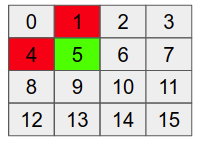
\includegraphics[scale=1]{fig/seidel_code.png}
		\caption{The read and write scheme in the input code}
		\label{fig:readWrite}
	\end{figure}
	
	\subsubsection{Transformed\_Seidel function}
		The transformed function recursively tile the input elements until it gets to the tile size of one. In figure~\ref{fig:transformed}, I showed the tiling scheme. This is one example of non-affine transformation.
	\begin{figure}[h!]
		\centering
		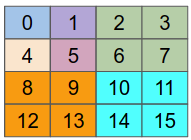
\includegraphics[scale=1]{fig/transformed.png}
		\caption{The recursive algorithm partitioning}
		\label{fig:transformed}
	\end{figure}

	\subsubsection{LastWriter}
	
	Line 84-90 checks the last statement instance that write into a specific data space. The procedure is as follows. First, it will get the write reference that is for a data space A[i][j] the write reference (wref) is (i,j) (line 87). Using the LHS\_MAP and wref\_fix\_flag, we drive the two inductive variables i and j in $S<t,i,j>$. Based on the original code in listing~\ref{code:original}, the last statement instance that writes into this specific data space is t = T - 1. They do this computation using the ISL library, which computes these faster using a specific data structure in the backend. However, for these small tests, I don't think that there would be a meaningful difference in the overhead of these assertions. Please see the listing~\ref{code:lastWriter} for further implementation details. Line 16-20 is the mapping part, and lines 23 to 29 drive the last writer statement instance. After doing this computation for each data space, we can ensure that the program is finished completely.


   \begin{lstlisting}[caption={The lastWriter fucntion}, label={code:lastWriter}, captionpos=b, numbers=left,
   stepnumber=1]
StateInst lastWriter(const StateInst& max_b,const std::vector<int>& wref,
const std::vector<bool>& fix_flags,const std::vector<std::vector<int>>& mapping){
	StateInst result;
	result.instance.resize(fix_flags.size());


	if(mapping.size() != wref.size()){
	std::cerr << "The mapping dimension doesn't match the wref dimentions" << std::endl;
	}
	
	if(std::count(fix_flags.begin(), fix_flags.end(), true) != wref.size()){
	std::cerr << "The number of fixed iterations doesn't match the flag indicator" << std::endl;
	}
	
	//Compute the fixed iteration space
	std::vector<int> fixed_iter_space(wref.size());
	for(int row = 0; row < wref.size(); row++){
		for(int col = 0; col < wref.size(); col++)
			fixed_iter_space[col] += mapping[row][col] * wref[col];
	}
	
	int cnt = 0;
	for(int i = 0; i < fix_flags.size(); i++){
		if(!fix_flags[i]){
			result.instance[i] = max_b.instance[i] - 1;
		} else {
			result.instance[i] = fixed_iter_space[cnt];
			cnt++;
		}
	}

	result.makeValid();
	result.makeNoInit();
	
	return result;
}
	\end{lstlisting}
	
	\subsection{Instrumented function}	
	Now we need to instrument the Transformed-Seidel function for runtime checks. First, we need to find the statement instance that we want to instrument. Then we are inserting the required checks, using the variables that we have just defined and functions with SageInterface. For example, I am using SageInterface::addTextForUnparser function for most of my instrumentation. I also use  SageInterface::insertStatementAfter occasionally. Here, I am more focused on explaining the details of the functions and their implementation rather than the compiler part since that part is more repetitive work.

	We first drive the wref (Line 5). Note that we don't care how "ilo" and "jlo"  are obtained, and we only care about the values of these two variables, and thus, I am using their string representation to define wref. Given the last statement instance written in A[ilo][jlo], which is store in shadow[ilo][jlo] we have two situations. It is either the first time we want to write in this data space, or it is one of the writes coming after a previous write into this data space. If it is the first time, we use firstWriter function (Line 8). The procedure of this function is similar to the lastWriter function. However, instead of using the max\_bound, we are using the min\_bound, and we are going back in time.
	
	
\begin{lstlisting}[caption={The instrumented code}, label={code:InstrumentedFunction}, numbers=left, captionpos=b, stepnumber=1]
void Instrumented_Seidel(int t,int ilo,int ihi, int jlo, int jhi){
if (ilo > ihi || jlo > jhi) return;
if (ilo == ihi && jlo == jhi){
 A[ilo][jlo] = A[ilo-1][jlo] + A[ilo][jlo-1];
 std::vector<int> wref{ilo, jlo};
 polyfunc::StateInst optStat;
 if(shadow[ilo][jlo].isInit() || !shadow[ilo][jlo].isValid()){
  optStat = polyfunc::firstWriter(min_bound, wref, wref_fix_flag, mapping.LHS_MAP);
  assert(optStat.isValid());
 } else {
  optStat = polyfunc::nextWriter(shadow[ilo][jlo], max_bound, wref, wref_fix_flag, mapping.LHS_MAP);
  assert(optStat.isValid());
 }

 //Checking the right hand side
 std::vector<int> read_ref{ilo - 1, jlo, ilo, jlo - 1};
 for(int rr_ptr = 0; rr_ptr < read_ref.size(); rr_ptr++){
 assert(polyfunc::dotProduct(mapping.RHS_MAP[rr_ptr], optStat.instance) + read_const[rr_ptr] == read_ref[rr_ptr]);
 }
 
 //Checking the validity of the value of rhs arrays
 std::vector<int> read_ref0(read_ref.begin(), read_ref.begin() + 2);
 assert(shadow[ilo - 1][jlo] == polyfunc::writeBeforeRead(optStat, min_bound, read_ref0, wref_fix_flag, mapping.LHS_MAP));
 std::vector<int> read_ref1(read_ref.begin() + 2, read_ref.begin() + 4);
 assert(shadow[ilo][jlo - 1] == polyfunc::writeBeforeRead(optStat, min_bound, read_ref1, wref_fix_flag, mapping.LHS_MAP));
 shadow[ilo][jlo] = optStat;
 //=======================================================
 
 
 }else{
	 Instrumented_Seidel(t, ilo,(ilo + ihi) / 2, jlo, (jlo + jhi)/2); //Top-Left
	 Instrumented_Seidel(t, ilo,(ilo + ihi) / 2, (jlo + jhi) / 2 + 1,jhi); //Top-Right
	 Instrumented_Seidel(t, (ilo + ihi) / 2 + 1, ihi, jlo, (jlo + jhi) / 2); //Bottom-Left
	 Instrumented_Seidel(t, (ilo + ihi) / 2 + 1, ihi, (jlo + jhi)/2 + 1, jhi); //Bottom-Right
 }
 

 if (ilo == 1 && ihi == N - 1 && jlo == 1 && jhi == N-1 && t < (T - 1)){ 
 	Instrumented_Seidel(t+1, ilo, ihi, jlo, jhi);// Next time step
 }
}
	\end{lstlisting}
	
	 If it is the second situation, we should use nextWriter function (Line 11). This function aims to get the previous statement instance that writes into this place and generate the next writer using the original schedule of the original program. For example, after seeing the statement instance $S<1,5,6>$, using the original schedule should generate $S<2,5,6>$ as the following statement instance that writes into this place. Please note that these functions are general, and we need to use wref and mapping to find the write statement instance. 

	Please see listing~\ref{code:nextWriter}. For simplicity, I removed some of the condition checks in the function. For the original implementation, please see the attached code. In lines 27-32, we will find the first inner loop that doesn't affect the wref. Then, we start by finding the first statement instance that writes into this specific place after the previous statement (line 34 to 42). If we find a valid statement instance, then we are good to go for the next step. 
		 
		 
\begin{lstlisting}[caption={nextWriter function}, label={code:nextWriter}, numbers=left, captionpos=b, stepnumber=1]
StateInst nextWriter(const StateInst& prev,const StateInst& max_b,const std::vector<int>& wref,
const std::vector<bool>& fix_flags, const std::vector<std::vector<int>>& mapping){
	StateInst result;
	result.instance.resize(fix_flags.size());
	result.makeNoInit();

	std::vector<int> fixed_iter_space(wref.size());
	for(int row = 0; row < wref.size(); row++){
		for(int col = 0; col < wref.size(); col++)
			fixed_iter_space[col] += mapping[row][col] * wref[col];
	}

	//Create the correct instance
	int cnt = 0;
	for(int i = 0; i < fix_flags.size(); i++){
		if(!fix_flags[i]){
			result.instance[i] = prev.instance[i];
		} else {
			result.instance[i] = fixed_iter_space[cnt];
			cnt++;
		}
	}

	//compute the nextwriter
	//Compute the place where incrimination begins
	int starting_point = 0;
	for(int i = 0; i < result.instance.size(); i++){
		if(fix_flags[i]){
			starting_point = i - 1;
			break;
		}
	}
	
	for(int i = starting_point; i >= 0; i--){
		int tmp = result.instance[i] + 1;
		if(tmp < max_b.instance[i]){
			result.instance[i] = tmp;
			result.makeValid();
			return result;
	} else {
		continue;
	}

	result.invalidate();
	return result;
}
\end{lstlisting}

		 After computing the statement instance, we know the correct statement that should write into this place right now. So, we have to check whether the current operation is equal to the computation of the statement instance that we just computed or not. In listing~\ref{code:InstrumentedFunction}, line 16-19. Using the RHS\_MAP drive from the original code, we are converting the iteration space of the statement instance that we drove into the read data space. Then we are checking these read data spaces with the read data space that is currently happening. If they are equal, we will go to the next step, checking the values of these data.
	
	In lines 22-26, we are using the last vital function writeBeforeRead. This function can reflect the use of mapping better. Here, we use the statement instance we just computed as a time reference, and we want to drive a statement instance that writes into some data space that occurs before the current statement instance. For example, assume that we are currently computing $S<1,5,7>$. The last statement instance that writes into A[4][7] is $S<1,4,7>$, and the last one that writes into data space A[6][7] is $S<0,6,7>$. In listing~\ref{code:writeBeforeRead} we first need to find the fixed inductive variables that always write into specific data space. Note that it is similar to nextWriter and lastWriter function. The only difference is that now we are working on reading references rather than wref. Please note that we still use the LHS\_MAP since the mapping for that specific statement instance that writes into the current read reference is the same. Also, please see lines 34-42 that show the going back in time.
	
\begin{lstlisting}[caption={writeBeforeRead function}, label={code:writeBeforeRead}, numbers=left, captionpos=b, stepnumber=1]

StateInst writeBeforeRead(const StateInst& current_read, const StateInst& min_b, const std::vector<int>& wread,
const std::vector<bool>& fix_flags, const std::vector<std::vector<int>>& mapping){
		assert(current_read >= min_b);
		StateInst result;
		result.makeNoInit();
		result.instance.resize(fix_flags.size());

	std::vector<int> fixed_iter_space(wread.size());
	for(int row = 0; row < wread.size(); row++){
		for(int col = 0; col < wread.size(); col++)
			fixed_iter_space[col] += mapping[row][col] * wread[col];
	}

	//Create the correct instance
	int cnt = 0;
	for(int i = 0; i < fix_flags.size(); i++){
		if(!fix_flags[i]){
			result.instance[i] = current_read.instance[i];
		} else {
		result.instance[i] = fixed_iter_space[cnt];
		cnt++;
		}
	}

	if(result < current_read){
		//It is a data form Input set that not yet being
		// written by any other statement instance
		for(int i = 0; i < result.instance.size(); i++){
			if(result.instance[i] < min_b.instance[i]){
				result.makeValid();
				result.makeInit();
				return result;
			}
		}
	
		result.makeValid();
		result.makeNoInit();
		return result;
	}

	//Compute the place where decrement begins
	int starting_point = 0;
	for(int i = 0; i < result.instance.size(); i++){
		if(fix_flags[i]){
			starting_point = i - 1;
			break;
		}
	}

	for(int i = starting_point; i >= 0; i--){
		int tmp = result.instance[i] - 1;
		if(tmp > min_b.instance[i]){
			result.instance[i] = tmp;
		} else {
		continue;
		}
	}

	//It is a data form Input set that not yet being
	// written by any other statement instance
	for(int i = 0; i < result.instance.size(); i++){
		if(result.instance[i] < min_b.instance[i]){
			result.makeValid();
			result.makeInit();
			return result;
		}
	}

	result.makeValid();
	result.makeNoInit();
	return result;
}

\end{lstlisting}
\section{Implementation of the Original Schedule and print statement in Compiler}

Although I am using a limited representation of the original schedule, and now a predefined function to print the statement and use these in the current implementation, but I have also implemented these function at the beginning from the scratch. 

Please see the figure~\ref{fig:graph} and its corresponding code in figure~\ref{fig:code}. In here, we can see that the tree is in levels and each levels defined by the statements and the level of nesting that they have. So, basically to extract the original schedule we need to drive these levels, and for each level, we will assign an statement instance shape. To do that, I am using "AstTopDownProcessing" to extract these information and for each SgExprStatement, we are adding the template using addNewAttribute function and attribute class to the nodes in the AST tree.


\begin{figure}[h!]
	\centering
	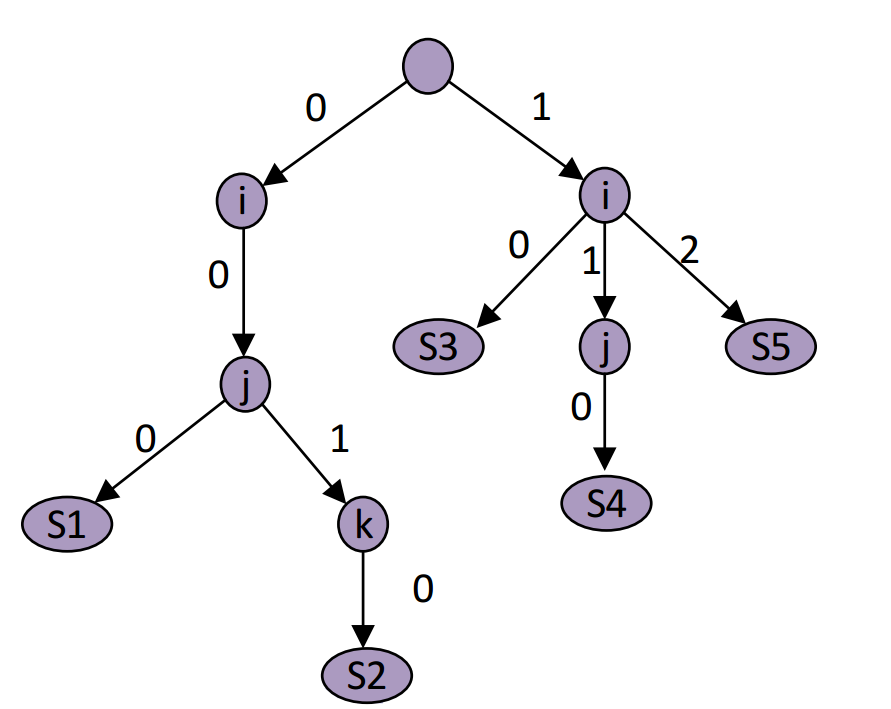
\includegraphics[scale=0.25]{fig/graph.png}
	\caption{The original schedule graph that shows the dependency between statement instances in an affine program}
	\label{fig:graph}
\end{figure}

\begin{figure}[h!]
	\centering
	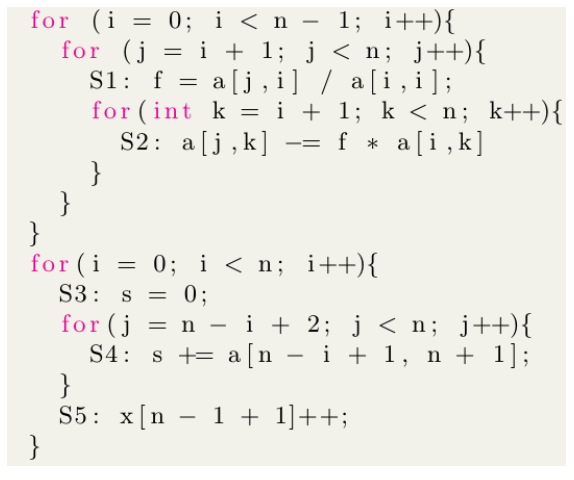
\includegraphics[scale=0.5]{fig/code.png}
	\caption{The toy example that we use to drive the original schedule of the program}
	\label{fig:code}
\end{figure}

For example, please consider statement S1. It is in the 2 nested for-loops. S1 shape is $S<0,i,0,j, 0>$ where the last 0 is its priority inside the basic block of the two nested loops. So, any statement in this 2 nested for loops will have $S<0,i,0,j>$ in their beginning. Using this information and the traversing method that I have mentioned, I have implemented a general original schedule retriever. 

As for the printing function, I implemented it using a AstBottomUpProcessing traversal. Then, each node will gather the string from its child in the AST tree and add its own string definition to it and parse it up in the AST. Please see listing~\ref{code:printing} for a detailed implementation.


\begin{lstlisting}[caption={Buttom up traversal - Based on the type of the node we will retrieving its string and pass it to its parent.}, label={code:printing}, numbers=left, captionpos=b, stepnumber=1]

std::string PrintSubscripts::evaluateSynthesizedAttribute(SgNode* node, SynthesizedAttributesList child_att){
	if(isSgBinaryOp(node)){
		if(isSgAddOp(node)){
			return child_att.front() + " + " + child_att.back();
		} else if(isSgSubtractOp(node)){
			return child_att.front() + " - " + child_att.back();
		} else if(isSgMultiplyOp(node)){
			return child_att.front() + " * " + child_att.back();
		} else if(isSgDivideOp(node)){
			return child_att.front() + " / " + child_att.back();
		}
	} else if(isSgValueExp(node)){
		if(isSgIntVal(node)){
			return std::to_string(isSgIntVal(node)->get_value());
		} else if(isSgDoubleVal(node)){
			return std::to_string(isSgDoubleVal(node)->get_value());
		} else if(isSgFloat128Val(node)){
			return std::to_string(isSgFloat128Val(node)->get_value());
		}
	} else if(isSgVarRefExp(node)){
		return isSgVarRefExp(node)->get_symbol()->get_name();
	} else {
		std::cerr << "This is not a valid subscript" << std::endl;
	}
	return "";
}

\end{lstlisting}


 
\section{A note about Algorithm B in the paper}

	If a statement instance can pass all of these tests, then it is a valid statement instance. There is one more algorithm in the paper. The terminology is the same. However, even with ISL, the overhead was huge, so they decided to work with numbers instead of integer sets. That is, for example, the statement instances that write into A[5][7] (like S<0,5,7>, S<1,5,7>, etc.) can be mapped into a sequence of numbers. They present some conditions that guarantee that this mapping exists, and then they use these sequences of numbers to check all those assertions.
	
	\section{Evaluation}
	
To test for this example, I change the boundaries of the recursive calls to see whether the Polycheck demo can detect the errors. It successfully detects these bugs while the test suit failed to generate errors. 

Unfortunately, as you have noticed, this implementation doesn't cover many corner cases. Since it is not integrated with the PoCC compiler, I could not check it with a benchmark, and I am sure that it will work with this example. As a hands-on experiment, I am happy that I could understand a small compiler research space and work with one scientific compiler. However, this implementation by no means is complete, and it cannot extends to general cases. But I did my best to grab the core idea of the PolyCheck paper.

As for the overhead, with T=3 and N=64 in the Seidel example, please see the runtime:
\begin{itemize}
	\item Time taken by Original\_Seidel: 8 microseconds
	\item Time taken by Transformed\_Seidel: 64 microseconds
	\item Time taken by Instrumented\_Seidel: 1548 microseconds
\end{itemize}

As we can see, the overhead is not that small! That is why they come up with algorithm B at the end. But, I believe that the bottleneck is also a direct cause of the use of the shadow variable itself rather than the computations alone.

To compile the code on Ubuntu, install ROSE using the official repo they have provided using the apt install command (it will not take a lot of time compared to compiling the rose from the source). Then please change the CMakeLists.txt based on the address of the library in your machine. If you want to see a demo, please go to the demo folder and use the "Project" executor with the address of your input code (Though I think it will not work because of some dynamic libraries that I have used). The rose\_* will be the instrumented code. Note that you should have a Transformed\_* function and an Original\_code* for instrumentation purposes in the input code. Please note that the header file polycheck\_demo\_functions.h should also be included since the instrumentation uses the function in this header file.
	
	\section{Discussion}
	
	As we discussed in the project presentation, the overhead of this implementation is enormous, and we cannot detect bugs until they happen!. The data also needs to move inside the same control flow, and if there are branches that depend on specific data, the verification will still be data-dependent. However, it is now more independent from the data than other testing technics that rely on the data results. It is a good technique for debugging since it can also approximately detect where the error is happening. Still, it cannot be used in sensitive works because of its overhead and that it will detect errors in the late stages. 


	Please note that the overhead of this technique is still much less than the previous trace-based work, namely CodeThorn.

	\section{Summary}
	\bibliography{references}
	\bibliographystyle{ieeetr}
	
	
\end{document}